SNO+ \cite{Kraus:2010zzb} is the follow-up of the successful SNO experiment \cite{SNO:1999crp}, located at SNOLAB, in Canada. It re-uses the existing equipment of the detector (acrylic vessel, photomultipliers and their support structure, electronics and the light water shield) replacing the heavy water by $\sim$780 tonnes of liquid scintillator (linear alkylbenzene, LAB).

The physics program of the SNO+ detector includes measurements of low energy solar neutrinos and \bbonu\ searches using \ND. In order to do that, the liquid scintillator will be loaded with a neodymium salt, resulting in about 50 kg of \ND. This isotope has the second highest endpoint, 3.37 MeV, and the fastest predicted neutrinoless double beta decay rate due to its large phase space factor, see fig.~\ref{fig:g0nu}. The high endpoint is above most radioactive backgrounds, such as radon, and this is a significant advantage. However, enrichment of this isotope seems difficult.

The energy resolution of the SNO+ detector is estimated to be 6.5\% FWHM at 3.4 MeV. External backgrounds can be rejected with a relatively tight fiducial volume selection, cutting however about 50\% of the signal. The most important sources of background are expected to be \TL\ impurities in the scintillator, the irreducible background from $^{8}$B solar neutrinos and \bbtnuº events from \ND . Assuming the radiopurity levels for the liquid scintillator achieved by BOREXINO ($\sim10^{-17}$ g/g of \TL) \cite{Borexino:2009awt}, simulations predict a background rate of $\sim10^{-2}$ \ckkbby\ \cite{Wright:2009csa}. 

The SNO+ experiment is expected to start commissioning in the spring of 2013 with pure liquid scintillator, to be followed by the Nd-loaded liquid scintillator phase. Given that the LAB liquid scintillator is about 15\%  less dense than the surrounding light water, one of the major technical challenges of the SNO+ upgrade is the design of a hold-down system for the acrylic vessel using a net of radiopure ropes, see fig.~\ref{fig:snoplus_anchor_possibility}.  

%%%%%
\begin{figure}[t!b!]
\begin{center}
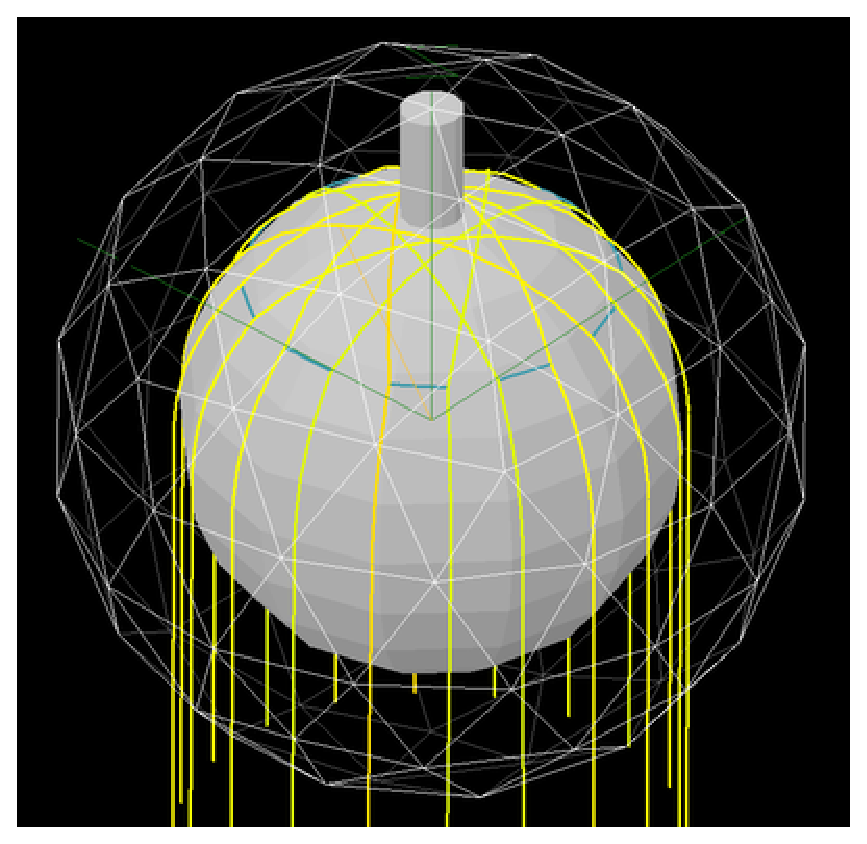
\includegraphics[width=0.55\textwidth]{img/Snoplus_anchor_possibility.eps}
\end{center}
\caption{\label{fig:snoplus_anchor_possibility}One of the candidate configurations for the SNO+ acrylic vessel anchor system. The acrylic vessel is shown in grey, and the anchor system in yellow. The outer sphere made of triangles is the PMT support structure.} 
\end{figure}
%%%%%